
\subsection{Configurazione utilizzo ADC}

\begin{figure}
	\centering
	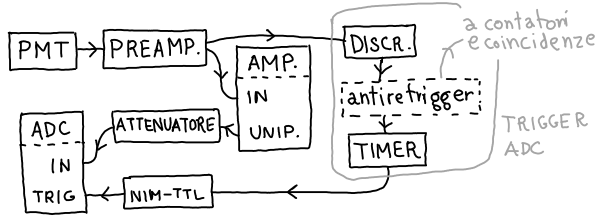
\includegraphics[width=28em]{schemaadc}
	\caption{\label{fig:schemaadc}
	Circuito per misurare l'energia rilasciata negli scintillatori.}
\end{figure}

\marginpar{Cambiare titolo in ``Misura del rilascio di energia''?}
La necessità di misurare quantitativamente il rilascio di energia nel rivelatore ci obbliga ad aggiungere nel nostro crate 3 moduli che permettono di digitalizzare l'uscita del PMT: il preamplificatore, l'amplificatore e l'ADC
(vedi circuito in \autoref{fig:schemaadc}).
Il preamplificatore ha il compito di allungare la durata dell'output del PMT dai nanosecondi ai microsecondi, in modo che l'amplificatore e l'ADC abbiano il tempo di leggerla. Esso è collegato direttamente al PMT che vogliamo usare per evitare riflessioni e non è possibile operare un adattamento di impedenza, in quanto il preamplificatore necessita di un'elevata impedenza d'ingresso per allungare la durata del segnale. 
Il~preamplificatore restituisce un segnale con una salita praticamente istantanea
ed una discesa esponenziale con un $\tau\approx\SI{15}{\mu s}$.

Il compito dell'amplificatore è intensificare il segnale al suo ingresso
(in questo caso quello del preamplificatore)
e restituire un'uscita analogica proporzionale all'energia del segnale in ingresso.
Ci sono due uscite analogiche che generano una forma diversa di segnale,
dette \emph{unipolare} e \emph{bipolare}.
Il manuale specifica che la forma dell'uscita unipolare
è data dalla funzione $e^{-3t}\sin^4{t}$ (simile a una gaussiana), in cui $t$ è il tempo.
La forma bipolare è simile ma ha il massimo anticipato rispetto a quello dell'unipolare.
La tensione massima in uscita è \SI{11}{V}.

Lo scopo dell'ADC è trasformare un segnale analogico in uno digitale
in modo che questo possa essere salvato su un computer.  
La conversione del segnale parte dopo circa \SI{1}{\micro s} dall'arrivo di un segnale di \emph{trigger} e dura all'incirca tale intervallo di tempo. L'ADC può leggere segnali analogici che vanno da qualche \si{mV} a \SI{3.3}{V} e può digitalizzarne al massimo 40 al secondo;
il trigger legge un segnale TTL a~\SI{3.3}{V}. La risoluzione della nostra ADC è a 12 bit.

Per poter sfruttare l'apparato di digitalizzazione dobbiamo trasformare l'uscita del PMT adoperando il preamplificatore,
attenuare il segnale dell'amplificatore in modo che non possa danneggiare l'ADC
e costruire un trigger che faccia partire l'acquisizione
in modo che l'ADC campioni il segnale sul massimo dell'uscita dell'amplificatore.
Per fare il trigger mettiamo un discriminatore sull'uscita del preamplificatore
e la ritardiamo con un timer.

\subsubsection{Taratura del trigger}

\begin{figure}
	\centering
	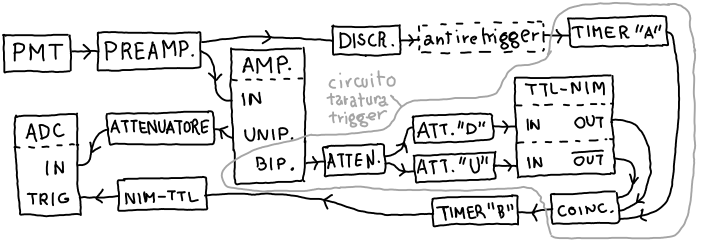
\includegraphics[width=0.9\textwidth]{schematrig}
	\caption{\label{fig:schematrig}
	Circuito per la taratura del timer del trigger dell'ADC.
	Il timer~A è regolato in modo che la coincidenza possa scattare
	solo in un certo istante del segnale in uscita bipolare dell'amplificatore.
	L'istante è stato scelto in modo da avere la massima pendenza del segnale
	per restringere la durata del segnale in uscita del discriminatore a doppia soglia.
	Per lo stesso motivo usiamo il bipolare anziché l'unipolare (ha una pendenza maggiore).
	Per eseguire la taratura modifichiamo la durata del timer~B
	cercando di massimizzare la lettura dell'ADC.
	Per tornare al circuito di misura (\autoref{fig:schemaadc}),
	togliamo la parte di taratura e colleghiamo in serie i timer A e B.}
\end{figure}

\marginpar{Aggiungere ``dell'ADC'' al titolo?}
La documentazione a disposizione dell'ADC non specifica esattamente
quanto tempo intercorre tra il segnale di trigger e il campionamento.
Per regolare il timer del circuito di trigger usiamo un circuito ausiliario
(vedi \autoref{fig:schematrig}).
L'idea è mandare in ingresso all'amplificatore segnali ad energia costante
e poi regolare la durata del timer del trigger massimizzando la lettura dell'ADC,
poiché dobbiamo campionare sul massimo.
Poiché la forma del segnale in ingresso influisce sull'allineamento temporale
dell'uscita con l'ingresso,
per essere sicuri di tarare correttamente il trigger
dobbiamo mandare in ingresso proprio i segnali che dobbiamo misurare.%
\footnote{Quindi, per esempio, non possiamo usare un impulsatore.}
Quindi, per avere segnali ad energia costante,
selezionamo direttamente i segnali in base all'uscita dell'amplificatore.
Vogliamo avere un discriminatore a doppia soglia%
\footnote{Discriminatore che ha uscita a livello alto quando la tensione in ingresso è compresa tra le due soglie.}
sull'uscita dell'amplificatore, con soglie piuttosto vicine,
in coincidenza con un timer ausiliario per leggere l'uscita dell'amplificatore
sempre nello stesso punto della forma del segnale.
Poiché non disponiamo di moduli in logica positiva,
costruiamo questo discriminatore sfruttando il fatto che il modulo \texttt{TTL-NIM}
non è altro che un discriminatore dove la soglia (positiva) è quella che distingue i livelli logici.
Per avere due soglie diverse
usiamo due attenuatori impostati con una differenza di attenuazione più piccola possibile.
\marginpar{Forse dobbiamo parlare qui del problema che il nostro trigger non è detto
triggeri come triggera l'amplificatore (da cui la foto incriminante).}
